\section{k-means++}

Instead of arbitrarily initializing cluster centers in Lloyd's k-means
algorithm, k-mean++ algorithm chooses a center with probability that
is proportional to $D^2$ weighting.

Here's Lloyd's k-means algorithm:
\begin{algorithm}[H]
  \caption{Lloyd's k-means Algorithm}
  \label{ladder-mechanism}
  \begin{algorithmic}[1]
    \renewcommand\algorithmicrequire{\textbf{input}}     
    \STATE Initialize k centers $C_1, C_2, \cdots, C_k$ arbitrarily
    from ($x_1,x_2, \cdots , x_n$)  
    \STATE Assign each $x_i$ to the closest $C_j$ (this creates a
    partition $P_1, P_2, \cdots, P_k$) 
    \STATE Re-compute centers $C_j=\frac{1}{|P_j|} \sum_{x_i\in P_j} xi$
    \STATE Repeat step 2-3 until centers don't change by too much    
  \end{algorithmic}
\end{algorithm}

\begin{fact}
  Solution to Lloyd's method for k-means can be arbitrarily worse from
  the optimal solution.
\end{fact}
\begin{lemma}
  At every step of the algorithm, the k-means cost can only improve.
\end{lemma}
\begin{proof}
  For step 2, observation that $x_i$ are assigned to closest center,
  if a point is assigned to other centers, cost would go up.
  
  For step 3: once partition fixed, center is assigned by
  $\frac{1}{|P_j|} \sum_{x_i\in P_j} xi$ .
\end{proof}
\textbf{Possible Improvement}:
\begin{itemize}
\item Choose centers uniformly at random:\\
  \textit{Example}: Suppose optimal solution has 3 clusters($P_1,P_2,
  P_3$). If $C_1$ is chosen from $P_1$ and $C_2$ choose from $P_2$,
  then probability choosing $C_3$ from $P_3$ is only $1/3$.
  
  Probability choosing centers from each optimal clusters is very low
  ("Coupon Collective Problem"). Average time of trials to achieve it
  is: $klogk$. If pick $klogk$ centers, then all clusters will be
  covered. Extra merging step should be taken to reduce cluster size
  to $k$. 
  $Cost$
\item Farthest-First Traversal:\\
  $$cost ~ \Omega(\xi^2n)$$
  Outliers will not work for this method.
\item Probalistic Farthest-First Traversal(\textit{k-means++ paper}):
  \begin{enumerate}
  \item Pick $c_1$ uniformly at random from $X$.
  \item Take a new center $c_i$, choosing $x_j$ with probability
    \[P_j:=d^2(x_j,C)/\sum_{j'\in X}d^2(x_{j'},C)\]
  \item Repeat Step 2 until we have $k$ centers $C$.
  \end{enumerate}
\end{itemize}
\begin{theorem}
  For the initialization done by $k$-means++ algorithm, the
  $\mathbb{E}cost(c)] \leq O(logk)opt$ 
\end{theorem}
\begingroup\leftskip4em
Notation of potential function $\phi$, for $A\subset X=\{x_1\cdots
x_n\}$:  
\par\endgroup
\begin{align*}			
  &\phi(A) = \sum_{a\in A} \min_{c_j\in C} ||a-c_j||^2\\
  &\phi = \phi = cost(c)\\
  &\phi_{opt}(A)=  \sum_{a\in A} \min_{c_j\in C_opt} ||a-c_j||^2\\
  &\phi_{opt} = \phi_{opt}(X)
\end{align*}
\begin{proof}[Conceptually proof.]
  \hfill	
  \begin{figure}[H]
    \centering
    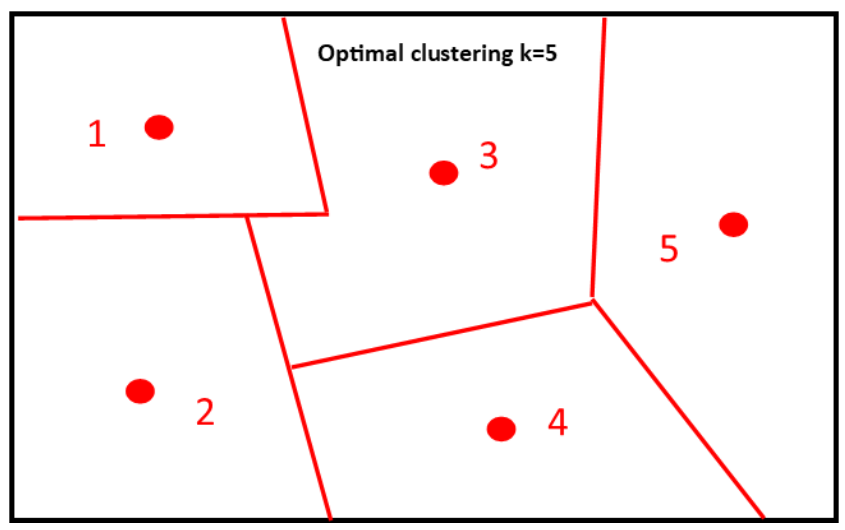
\includegraphics[width=0.8\textwidth]{chapter_1/files/optimal_clustering.png}
    \caption{\small Optimal Clustering with $k=5$}
  \end{figure}			
  \begin{enumerate}
    \begingroup\leftskip4em
  \item[agenda 1.] if the first pick falls under region 2, what
    expected cost for region 2 would be? 
  \item[agenda 2.] if some points are already picked, what expected
    cost for a particular region would be for next pick? 
    \par\endgroup
  \end{enumerate}			
\end{proof}
\begin{lemma}[Lemma 3.2 in $k$-means++ paper]
  Let $A$ be a cluster from $C_{opt}$, let $C$ be just one cluster
  chosen uniformly at random from $A$. Then $\mathbb{E}[\phi(A)]\leq
  2\phi_{opt}(A)$. 
\end{lemma}
\begin{proof}
  \hfill
  \begin{align*}
    \mathbb{E}[\phi(A)] &=\frac{1}{|A|}\sum_{a_0\in A}\sum_{a\in
      A}||a-a_0||^2, \ a_0\text{ is a center that chosen uniformly at
      random from}\ A\\ 
    &= \frac{1}{|A|}\sum_{a_0\in A, a\in
      A}||a-a_0||^2,\  (\textit{recall that
    }\mathbb{E}[||x-y||^2]=2\mathbb{E}[||x-\mathbb{E}(x)||^2])\\ 
    &=2\sum_{a \in A} ||a-\frac{1}{|A|}\sum_{a \in A}a||^2\\
    &=2\sum_{a \in A} ||a-c(A)||^2\\
    &\leq2\phi_{opt}(A)
  \end{align*}
\end{proof}
\begin{lemma}[Lemma 3.3 in $k$-means++ paper]
  Let $A$ be an arbirary cluster from $C_{opt}$ and $C$ be some
  arbitrary clustering. If we add a random center to $C$ ($C$ is a set
  of centers) from $A$ according to $k$-means++ weighting, then
  $\mathbb{E}[\phi(A)]\leq 8\phi_{opt}(A)$. 
\end{lemma}
\begin{proof}
  \underline{Observation}: probability that $a_0\in A$ is chosen:
  $D^2(a_0)/\sum_{a\in A}D^2(a)$, where $D^2(a_0)= d^2(a_0,C)$ and
  $D(a_0)$ denotes the shortest distance from $a_0$ to the closest
  center we have already chosen.
  
  For a given point $a\in A$, after choosing the center $a_0$, the
  contribution of $a$ to the cost will be $min(D^2(a),
  ||a-a_0||^2)$.\\ 
  \begin{align*}
    \mathbb{E}[\phi(A)] &= \sum_{a_0\in A}\frac{D^2(a_0)}{\sum_{a\in
        A}D^2(a)}\sum_{a\in A} min(D^2(a), ||a-a_0||^2)    \\
    D(a_0)&\leq D(a)+||a-a_0||, \forall a,a_0\\
    D^2(a_0)&\leq (D(a)+||a-a_0||)^2\\
    &\leq 2D^2(a)+2||a-a_0||^2\\
    \sum_{a\in A}D^2(a_0)&\leq 2\sum_{a\in A}(D^2(a)+||a-a_0||^2)\\ 
    D^2(a_0)&\leq \frac{2}{|A|}\sum_{a\in
      A}D^2(a)+\frac{2}{|A|}\sum_{a\in A}||a-a_0||^2\\\\ 
    \mathbb{E}[\phi(A)] &\leq \frac{2}{|A|}\sum_{a_0\in
      A}\frac{\sum_{a}D^2(a)}{\sum_{a}D^2(a)}\sum_{a\in A} min(D^2(a),
    ||a-a_0||^2)\ + \\ 
    &\hspace{1.5em} \frac{2}{|A|}\sum_{a_0\in
      A}\frac{\sum_{a}||a-a_0||^2}{\sum_{a}D^2(a)}\sum_{a\in A}
    min(D^2(a), ||a-a_0||^2)\\ 
    &\text{\textit{(pick}}\ ||a-a_0||^2\ \text{\textit{for the first
        term and pick}}\ D^2(a)\ \text{\textit{for the second
        term.)}}\\ 
    &\leq \frac{4}{|A|}\sum_{a_0\in A}\sum_{a}||a-a_0||^2\\
    &\leq 4\cdot 2\phi_{opt}(A)=8\phi_{opt}(A)
  \end{align*}	
\end{proof}
\begin{lemma}[Lemma 3.4 in $k$-means++ paper]
  Let $C$ be any arbitrary clustering we have chosen, choose $u>0$
  (number of uncovered clustering from $C_{opt}$). The corresponding
  uncovered points are $\chi_u$. Let $\chi_c=\chi-\chi_u$.\\\\ 
  \begin{figure}[H]
    \centering
    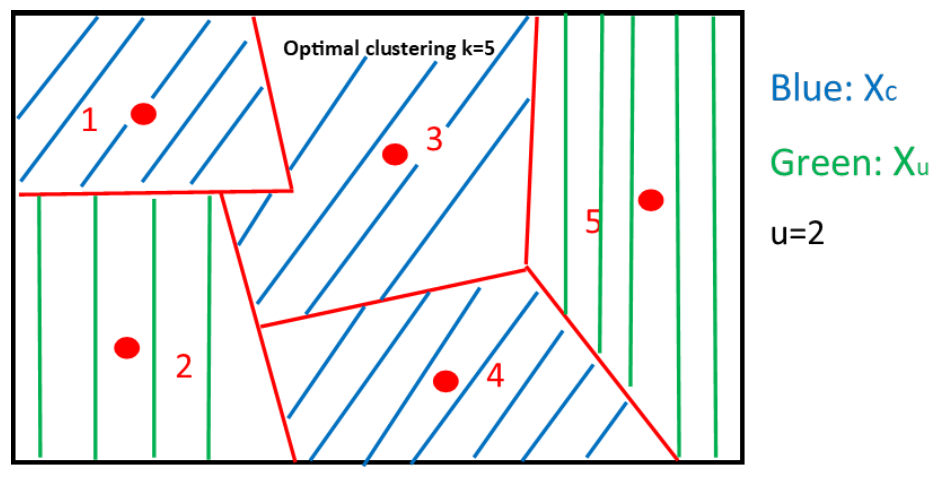
\includegraphics[width=0.8\textwidth]{chapter_1/files/pick_from_uncovered_points.png}
    \caption{\small Optimal Clustering with $k=5$}
  \end{figure}
  Now suppose we add $t\leq u$ random centers (according to
  $k$-means++) and $C'=C\cup\{c_1,c_2\cdots, c_t\}$. The corresponding
  cost is $\phi'$.\\ 
  $$\E[\phi']\leq(\phi(\chi_c)+8\phi_{opt}(\chi_u))(1+H_t)+\frac{u-t}{u}\phi(\chi_u)$$ 
  $$H_t=1+\frac{1}{2}+\frac{1}{3}+\cdots+\frac{1}{t}\ \text{is the harmonic sum}$$
\end{lemma} 
Let $A$ be the cluster which is covered by the first pick. Then
$u=k-1$, chose $t=k-1$ 
\begin{align*}
  \E[\phi']&\leq(\phi(A)+8\phi_{opt}(\chi-A)(1+H_{k-1}),\ (where\ H_{k-1}=2+\log
  k)\\ 
  &= (\phi(A)+8\phi_{opt}-8\phi_{opt}(A))(2+\log k),
  (where\ \phi(A)\leq2\phi_{opt}(A))\\  
  &\leq(2+\log k)8\phi_{opt}		
\end{align*}
\begin{proof}
  The proof was done by induction, showing that if we can prove
  equations $P(u,t-1)$ and $P(u-1,t-1)$ hold true, then $P(u,t)$ holds
  true. Base case of the induction is $P(u,0)\ for\ u>0$ and
  $P(1,1)$. 
\end{proof}
Example: Let $k=3$ for optimal clustering, after first pick there are
2 uncovered clusters from $C_{opt}$. Now we want to prove that
$P(2,2)$ holds true when we pick other two centers with $D^2$
weighting. By induction, if we prove that $P(2,1)$ and $P(1,1)$ hold
true then the result holds.  
	
\begin{algorithm}[H]
  \caption{Local Swap Algorithm}
  \label{ladder-mechanism}
  \begin{algorithmic}[1]
    \renewcommand\algorithmicrequire{\textbf{input}} 
    \REQUIRE ${x_1\cdots x_n}$, $k\in N$   
    \STATE Pick $T\subset \{x_1\cdots x_n\},\ |T|=k$ 
    \STATE Swap $t_i\in T$ with $x_j\in X$ if it improves the k-means cost.
    \STATE Repeat step 2 until no more improvement can be made.
  \end{algorithmic}
\end{algorithm}
\begin{lemma}[w/o proof]
  The solution to "local swap method" is no more than 25 optimum.
\end{lemma}
$$\text{k-means++ \& Lloydss }\sim O(logk)\cdot OPT$$
$$\text{Local Swap Method }\sim 25\cdot OPT$$
	
